\documentclass[a4paper]{article}
\usepackage[utf8]{inputenc}
\usepackage[russian]{babel}
\usepackage[T2]{fontenc}
\usepackage[warn]{mathtext}
\usepackage{graphicx}
\usepackage{amsmath}
\usepackage{floatflt}
\usepackage[left=20mm, top=20mm, right=20mm, bottom=20mm, footskip=10mm]{geometry}


\graphicspath{ {images/} }
\usepackage{multicol}
\setlength{\columnsep}{2cm}


\begin{document}

\begin{titlepage}
	\centering
	\vspace{5cm}
	{\scshape\LARGE Московский физико-технический институт \par}
	\vspace{5cm}

	{\huge\bfseries Растровый электронный микроскоп \par}

	\vspace{1cm}
	{\scshape\Large Лабораторная работа по курсу <<Вакуумная электроника>>\par}
	\vspace{1cm}
	\vfill
\begin{flushright}
	{\large выполнила студентка 653 группы ФФКЭ}\par
	\vspace{0.3cm}
	{\LARGE Карпова Татьяна Кирилловна} \par

	
\end{flushright}
	

	\vfill

% Bottom of the page
	Долгопрудный, 2018 г.
\end{titlepage}


\section{Цель работы}
\begin{enumerate}
    \item Изучить физические принципы функционирования и основные методики измерений РЭМ
    \item Получить изображения различных образцов в следующих режимах работы РЭМ:
    \begin{itemize}
        \item режим сбора истинно вторичных электронов
        \item режим сбора упруго-отражённых электронов
    \end{itemize}
\end{enumerate}

\section{Физические основы растровой электронной микроскопии}
Принцип растровой электронной микроскопии состоит в сканировании исследуемой поверхности тонким электронным лучом по типу телевизионной развёртки. Выбитые электронным лучом вторичные электроны регистрируются детектором электронов. Интенсивность полученного с детектора сигнала определяет яркость точки растра на итоговом изображении. Так как коэффициент вторичной эмиссии зависит от угла падения первичных электронов, на экране монитора возникает изображение, определяемое рельефом исследуемой поверхности.
\subsection{Вторичная электронная эмиссия}


\textbf{Вторичная электронная эмиссия} - испускание электронов из твёрдого тела при бомбардировке пучком первичных электронов. Это явление представляет собой сложное наложение нескольких взаимосвязанных процессов: упругое и неупругое рассеяние первичных электронов, возбуждение внутренних, истинно вторичных электронов, их движения к поверхности и выхода в вакуум. Сложный характер явления вторичной электронной эмиссии проявляется в энергетическом спектре вторичных электронов (рис. 1)

\begin{figure}[h]
\begin{center}
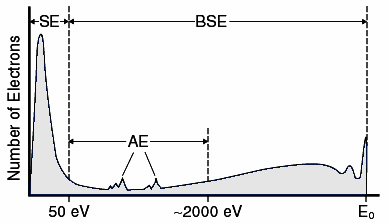
\includegraphics[width=10cm]{Electron_Spectrum.jpg}
\caption{Энергетический спектр вторичных электронов}
\label{ris:experimoriginal} %% метка рисунка для ссылки на него
\end{center}
\end{figure}

\begin{itemize}
    \item первая область ($<50$ eV) - медленные истинно вторичные электроны (secondary electrons).
    \item вторая область ($50 - 2000$ eV) - оже-электроны (Auger electrons) среди неупруго- и упруго-отражённых электронов (backscattered electrons)
    \item При энергии, близкой к энергии первичных электронов $E_0$, наблюдается узкий пик, соответствующий упруго отраженным электронам
\end{itemize}
Спектр \textbf{истинно вторичных электронов} имеет вид кривой с максимумом при некотором значении $E = E_m$. У металлов и полупроводников $E_m = 1.5 - 3$ эВ, полуширина спектра $\triangle E = 3 - 10$ эВ; у диэлектриков $E_m \approx 1$ эВ, полуширина спектра $\triangle E \approx 1.5 - 3$ эВ. Вторичная электронная эмиссия характеризуется коэффициентом вторичной эмиссии $\delta$, зависящим от элементного состава вещества и от угла падения пучка, то есть от рельефа поверхности. В частности, области на поверхности образца, на которые сканирующий пучок будет попадать под острыми углами, будут на изображении в РЭМ более светлыми. \par
В РЭМ также анализируются \textbf{отражённые электроны}. Коэффициент отражения - сложная функция $E_0$ и атомного номера $Z$ вещества. Если для малых энергий $E_0 = 0.6 - 3$ эВ для всех элементов максимум функции распределения соответствует упругоотражённым электронам, то для энергий $E_0 = 10 - 30$ кэВ максимум с ростом $Z$ растёт по величине и смещается в сторону $E_0$. При нормальном падении первичного пучка для всех элементов с ростом угла отражения уменьшается число отраженных электронов и сама величина максимума распределения.
\subsection{Контраст в растровом электронном микроскопе}
Информативными являются как отражённые, так и вторичные электроны. \par
Если образец однороден по составу и имеет выраженный рельеф, то изображение в \textbf{отражённых электронах} будет иметь такой же вид, как если бы мы смотрели на поверхность со стороны падения первичного пучка. Изображение также лишено полутонов и имеет чётко выраженные тёмные и светлые области. Для анализа образца, неоднородного по рельефу и составу, может использоваться парный детектор. \par
В отличие от отражённых электронов, изображение в \textbf{истинно вторичных электронах} содержит полутона и имеет гораздо больше деталей, следовательно является более привычным для человеческого глаза. Большая глубина фокуса в РЭМ обусловлена тем, что между объектом и детектором вторичных электронов нет линзы с осесимметричным полем (в оптическом микроскопе линза между объектом и глазом присутствует).
\subsection{Рентгеновский микроанализ}
Рентгеновский микроанализ в РЭМ осуществляется на основе следующих физических закономерностей и явления:
\begin{itemize}
    \item \textit{Закон Мозли} - зависимость энергии характеристического излучения от квадрата атомного числа элемента
    \item \textit{Явление электронного удара} - электрон пучка с энергией несколько кэВ выбивает из атома К-электрон (или переводит его на один из высоких свободных уровней), образуя вакансию. На образовавшуюся незанятую оболочку переходит один из L- или M-электронов, испуская рентгеновский фотон. 
\end{itemize}

\section{Устройство и работа электронного растрового электронного микроскопа}

\begin{figure}[h]
\begin{center}
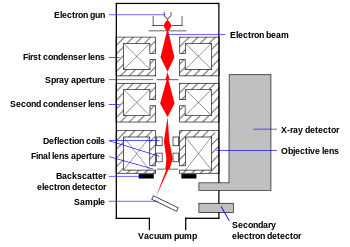
\includegraphics[width=12cm]{Schema_MEB_(en).png}
\caption{Общая схема растрового электронного микроскопа}
\label{ris:experimoriginal} %% метка рисунка для ссылки на него
\end{center}
\end{figure}

Структурная схема растрового электронного микроскопа представлена на рис. 2. Ускорение и фокусировка пучка происходит в колонне, вверху которой находится электронная пушка, испускающая электроны. Далее следует система электронной оптики, которая формирует узки зонд, а также позволяет отклонять его в сторону, направляя в определенные точки образца. Во внутренних областях колонны поддерживается вакуум, чтобы избежать рассеяния электронов и окисления вольфрамовой нити, являющейся источником электронов. Образец, крепящийся в специальном держателе, окружен детектирующей аппаратурой - детектором отражённых электронов, детектором вторичных электронов, рентгеновским спектрометром.
\begin{itemize}
    \item эмиссия электронов в приборе осуществляется \textit{термоэлектронным катодом} из вольфрамовой проволоки
    \item далее электроны разгоняются до энергий до 30 кэВ с помощью системы из анода и катода
    \item пройдя через отверстие в анодной пластине, электроны попадают в \textit{систему электромагнитных линз}, с помощью которых формируется узкий зонд. Система представляет собой цилиндрически симметричный электромагнит с очень острыми кольцевыми наконечниками полюсов, создающими сильное неоднородное магнитное поле, фокусирующее электроны
    \item С помощью системы \textit{отклоняющих электромагнитных катушек} происходит сканирование пучка по поверхности образца
    \item \textit{детектор вторичных электронов} представляет собой сцинцилляторный счётчик. Вторичные электроны собираются у детектора с помощью клетки Фарадея. Падающие на напылённый фосфором слой электроны вызывают испускание ультрафиолетовых фотонов, которые по световоду попадают в фотоумножитель
    \item для детектирования \textit{отражённых электронов} используется твердотельный детектор 
    \item для проведения рентгеновского микроанализа образца используются \textit{волновые или дисперсионные детекторы} рентгеновского излучения
\end{itemize}

\clearpage

\section{Выполнение работы}
\begin{enumerate}
    \item Получим изображение образца медь-хром в различных режимах работы микроскопа: в режиме сбора истинно вторичных электронов (SE) и в режиме сбора упругоотражённых электронов (BSE) (рис. 3 - 5)
    
    \begin{figure}[h]
\begin{center}
\begin{minipage}[h]{0.45\linewidth}
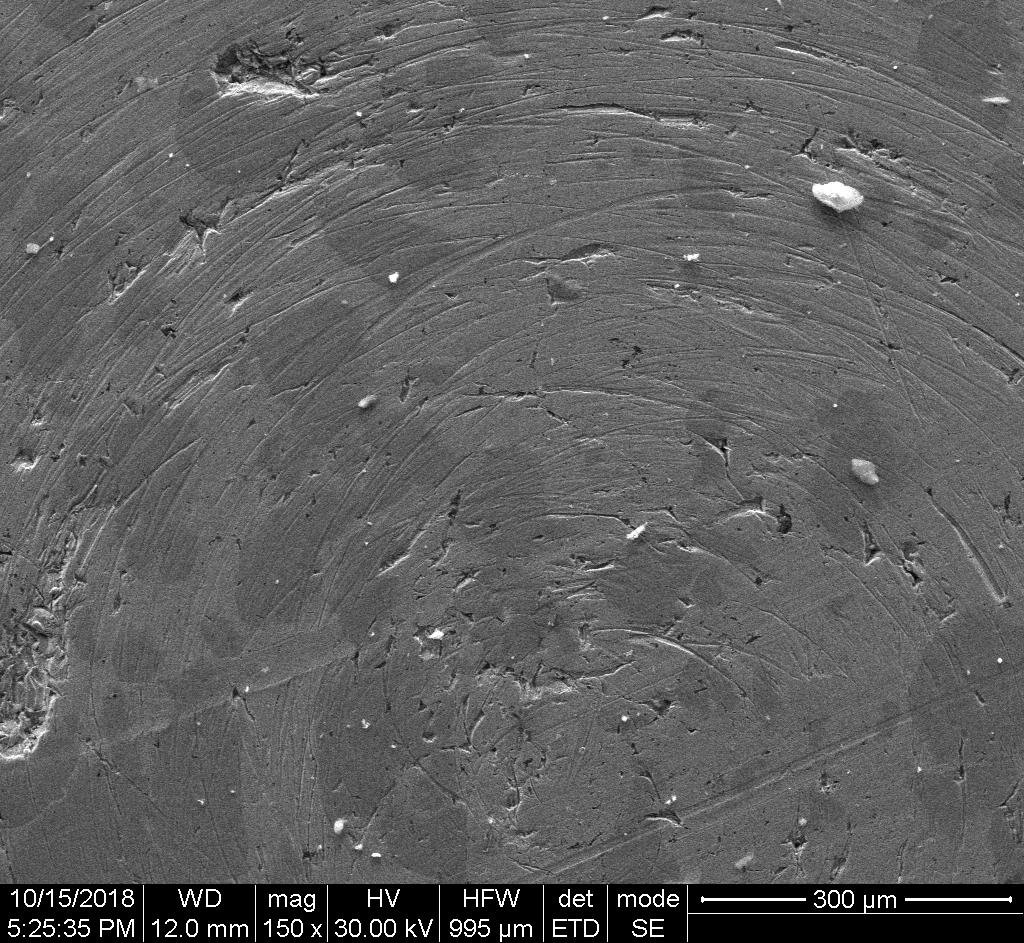
\includegraphics[width=1\linewidth]{iv1.jpg}
\caption{Изображение образца медь-хром (режим SE)} %% подпись к рисунку\label{ris:experimoriginal} %% метка рисунка для ссылки на него
\end{minipage}
\hfill 
\begin{minipage}[h]{0.45\linewidth}
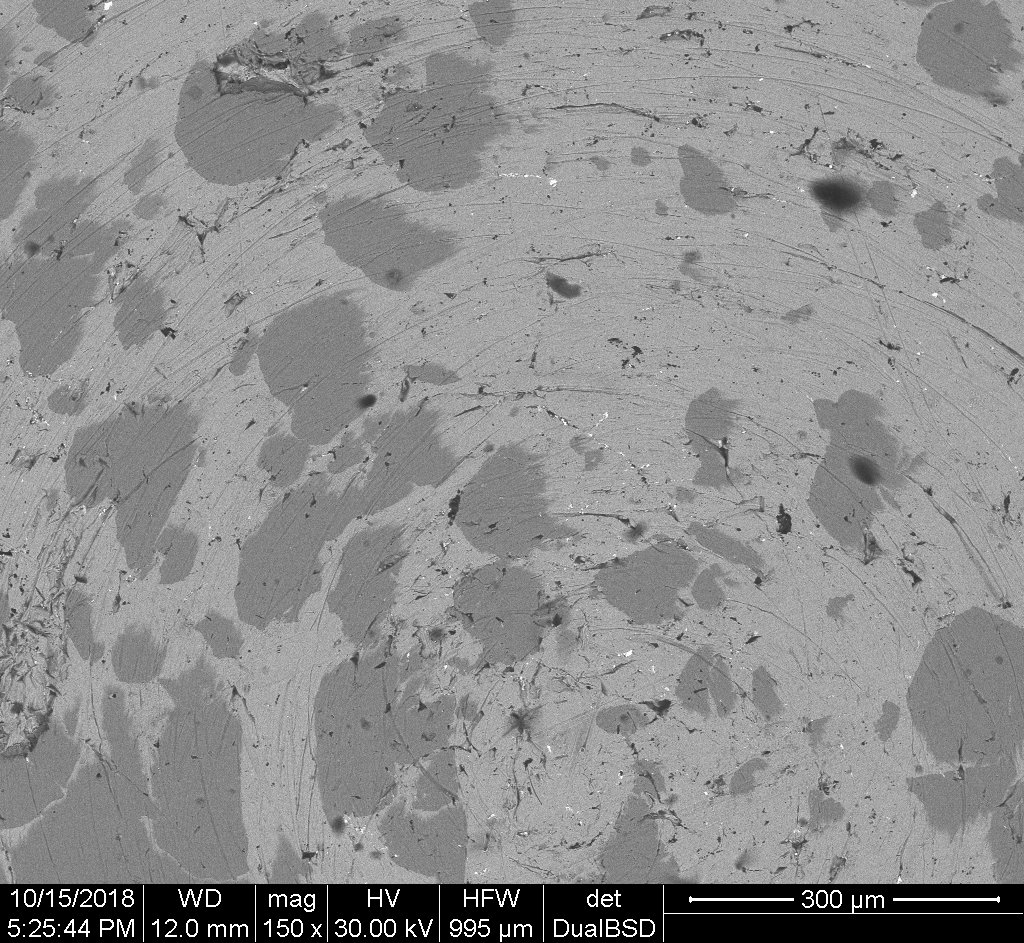
\includegraphics[width=1\linewidth]{z1.jpg}
\caption{Изображение образца медь-хром (элементный анализ, режим BSE)}
\label{ris:experimcoded}
\end{minipage}
\end{center}
\end{figure}

\begin{figure}[h]
\begin{center}
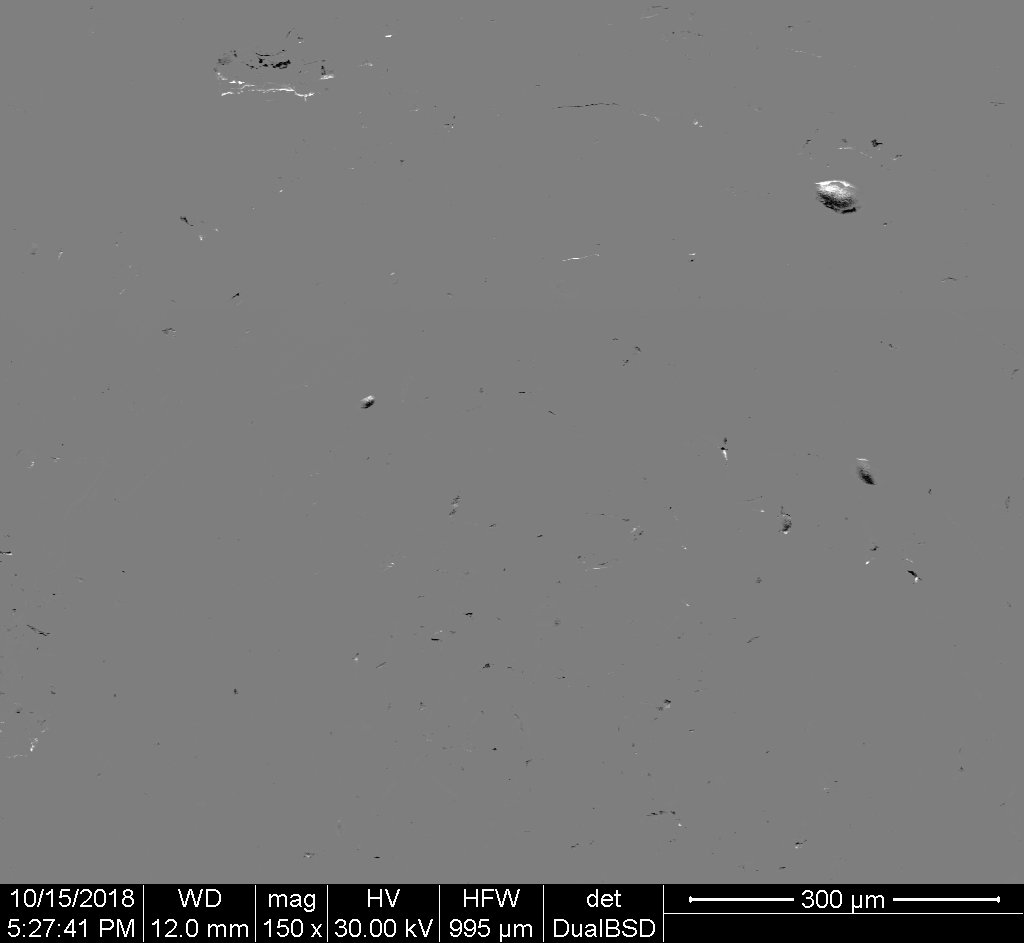
\includegraphics[width=7cm]{topo1_001.jpg}
\caption{Изображение образца медь-хром (топографический анализ, режим BSE)}
\label{ris:experimoriginal} %% метка рисунка для ссылки на него
\end{center}
\end{figure}

Проанализируем изображения. На первом изображении в истинно вторичных электронах представлен рельеф поверхности, присутствуют полутона. В отличие от него, на втором и третьем изображениях неровности отображены чёткими тёмными и светлыми пятнами. На первом и втором изображениях видны неоднородности образца по элементному составу. Заряд меди больше чем заряд хрома, и коэффициент отражения для неё больше при одинаковой энергии первичных электронов. Поэтому участки меди выглядят на изображении более светлыми, чем участки хрома. Третье изображение - чисто топографический анализ поверхности в отражённых электронах.

\clearpage 

\item Получим изображение микросхемы операционного усилителя в режиме сбора истинно вторичных электронов и в режиме сбора упругоотражённых электронов в разных масштабах и при разном времени выдержки (рис. 6 - 11).

    \begin{figure}[h]
\begin{center}
\begin{minipage}[h]{0.45\linewidth}
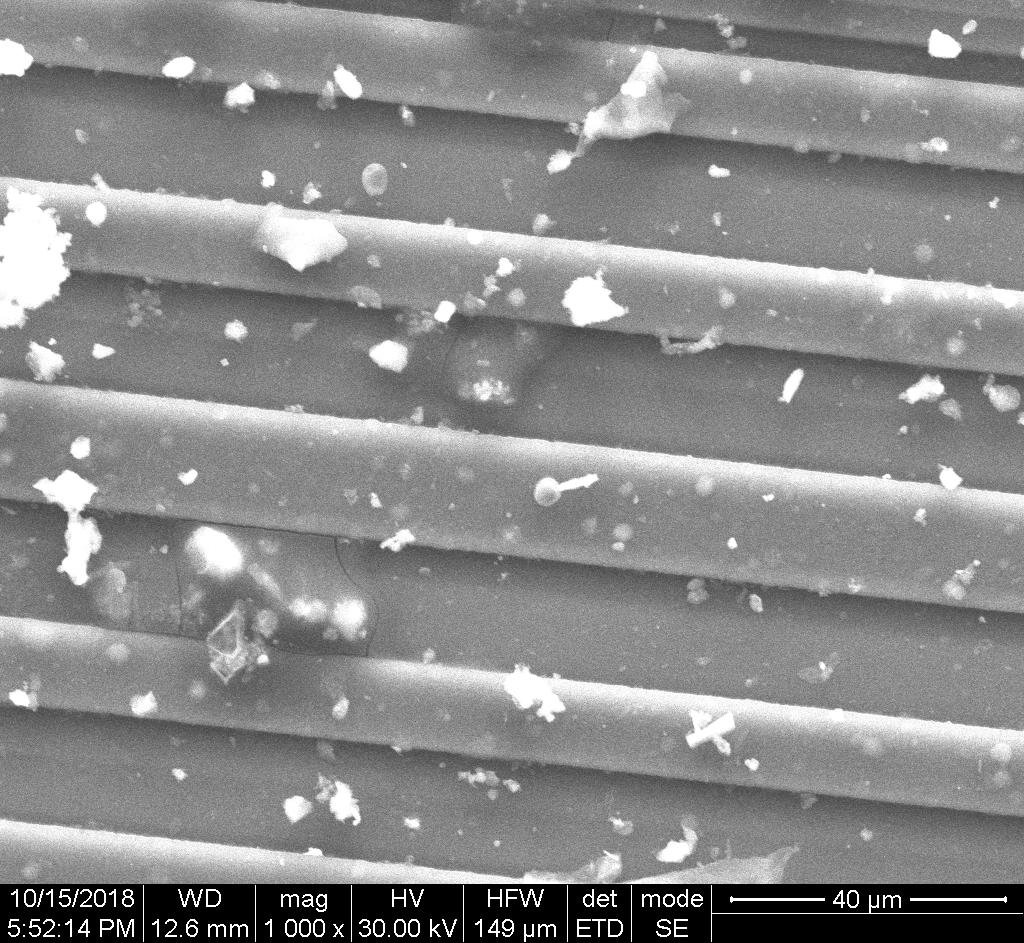
\includegraphics[width=1\linewidth]{iv1mikroch_002.jpg}
\caption{Изображение микросхемы (режим SE, увеличение 1000х)} %% подпись к рисунку\label{ris:experimoriginal} %% метка рисунка для ссылки на него
\end{minipage}
\hfill 
\begin{minipage}[h]{0.45\linewidth}
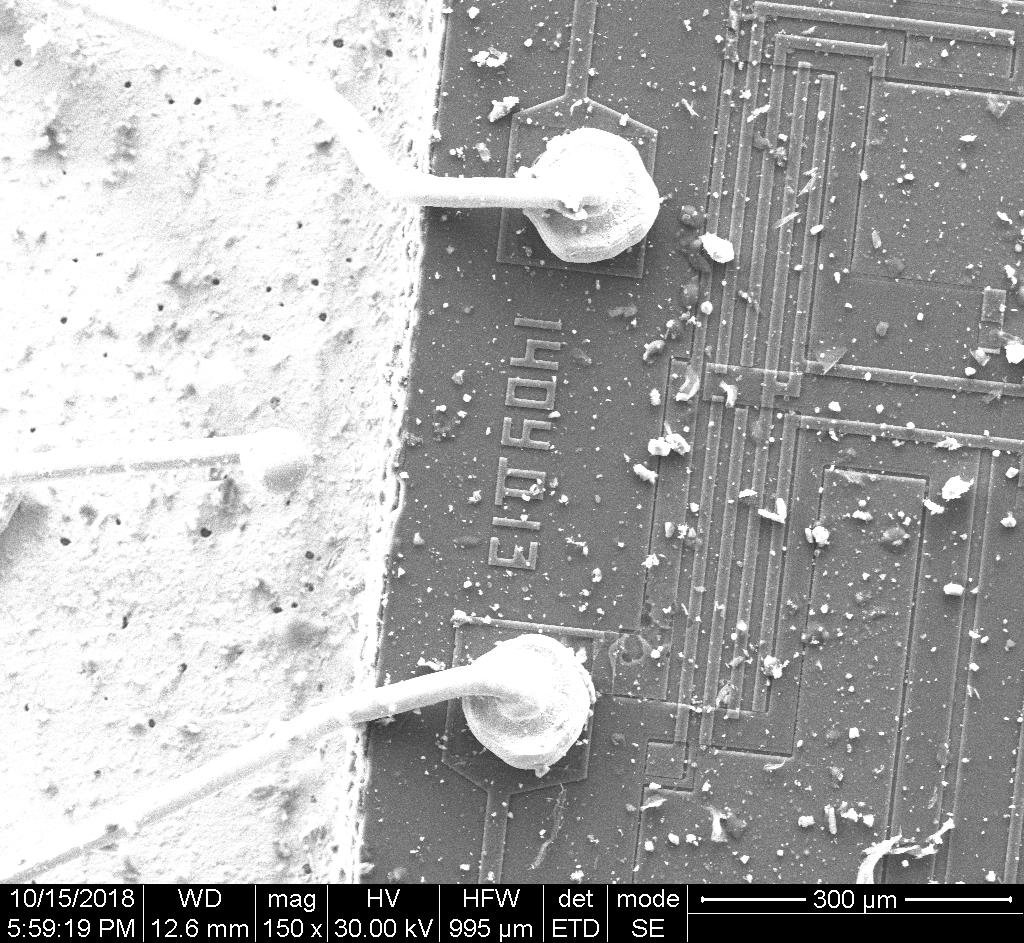
\includegraphics[width=1\linewidth]{iv1mikroch_004.jpg}
\caption{Изображение микросхемы (режим SE, увеличение 150х)}
\label{ris:experimcoded}
\end{minipage}
\end{center}
\end{figure}

    \begin{figure}[h]
\begin{center}
\begin{minipage}[h]{0.45\linewidth}
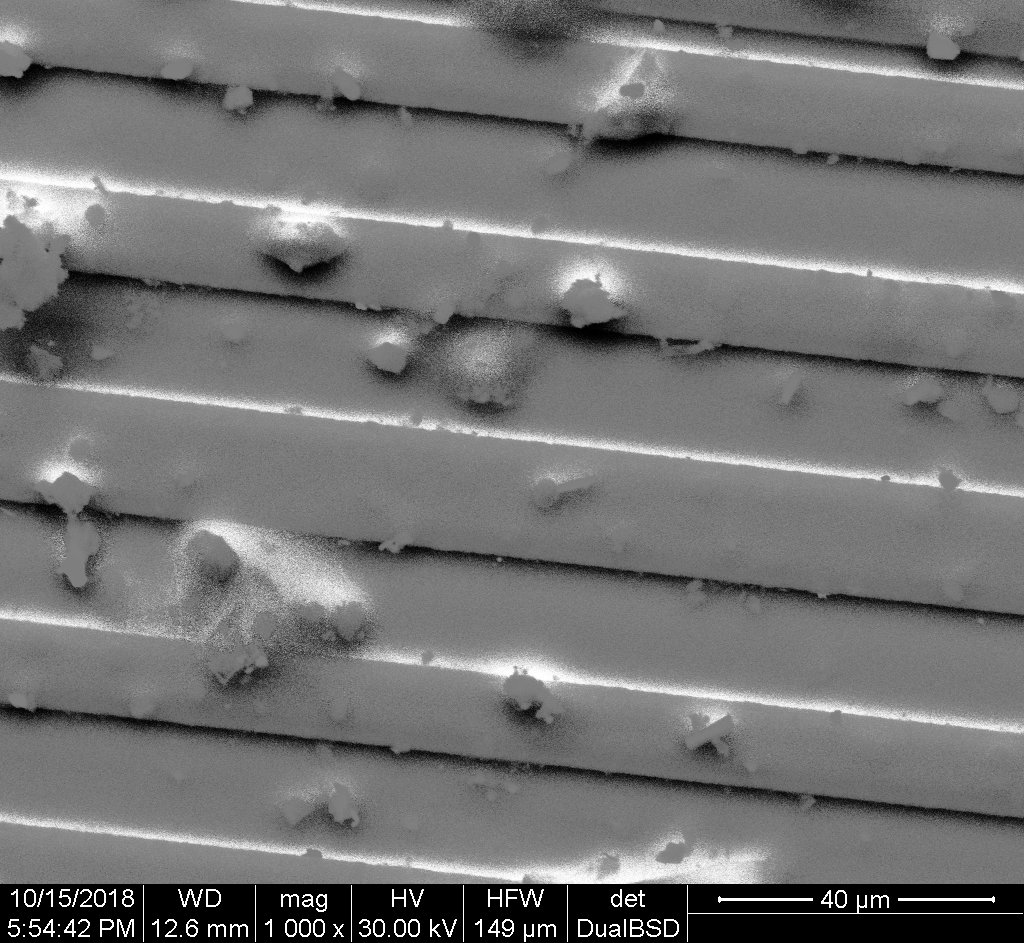
\includegraphics[width=1\linewidth]{topo1mikoch_005.jpg}
\caption{Изображение микросхемы (топографический анализ, режим BSE, увеличение 1000х)} %% подпись к рисунку\label{ris:experimoriginal} %% метка рисунка для ссылки на него
\end{minipage}
\hfill 
\begin{minipage}[h]{0.45\linewidth}
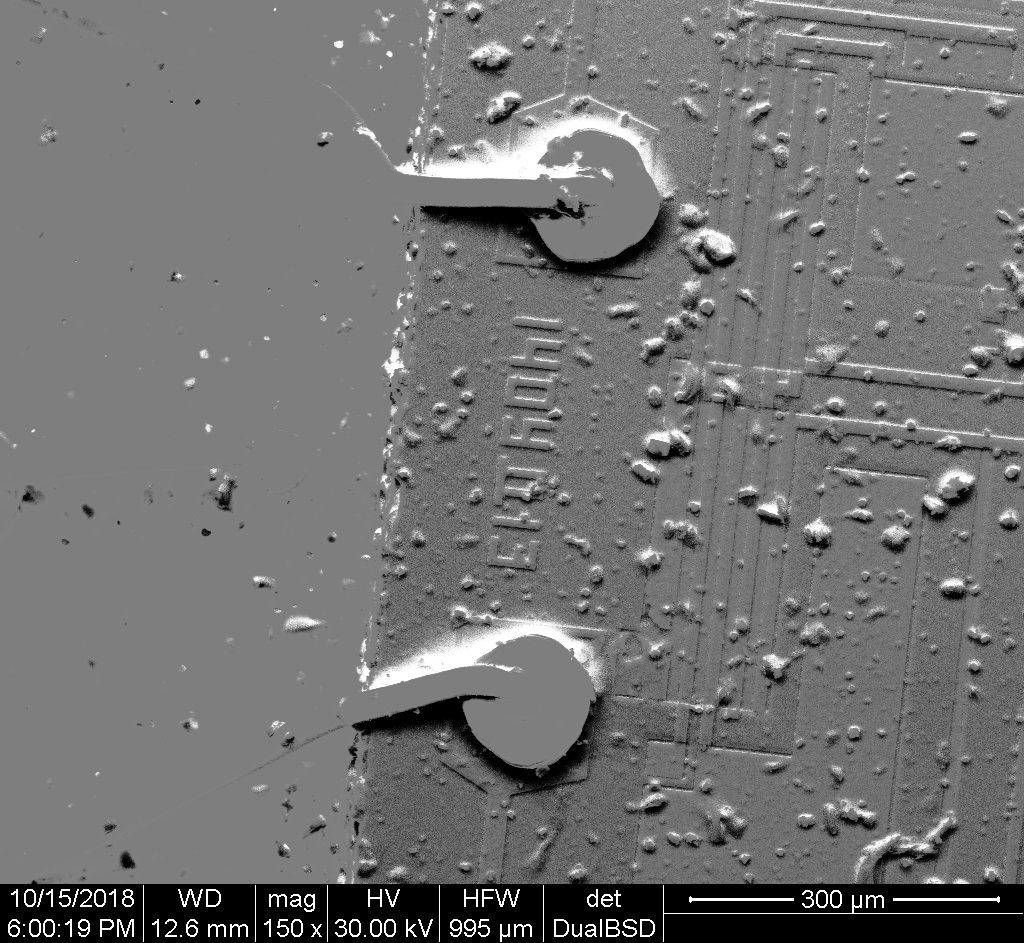
\includegraphics[width=1\linewidth]{topo1mikoch_008.jpg}
\caption{Изображение микросхемы (топографический анализ, режим BSE, увеличение 150х)}
\label{ris:experimcoded}
\end{minipage}
\end{center}
\end{figure}

    \begin{figure}[h]
\begin{center}
\begin{minipage}[h]{0.45\linewidth}
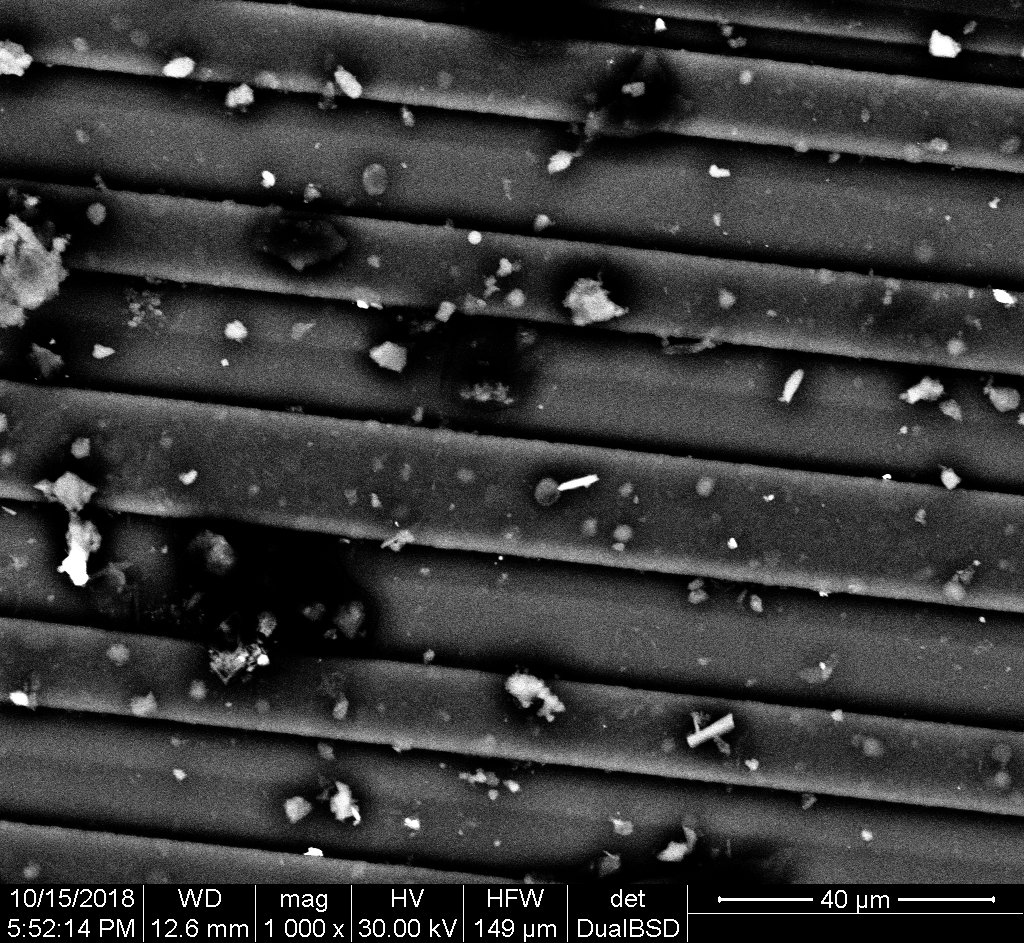
\includegraphics[width=1\linewidth]{z1mikoch_004.jpg}
\caption{Изображение микросхемы (элементный анализ, режим BSE, увеличение 1000х)} %% подпись к рисунку\label{ris:experimoriginal} %% метка рисунка для ссылки на него
\end{minipage}
\hfill 
\begin{minipage}[h]{0.45\linewidth}
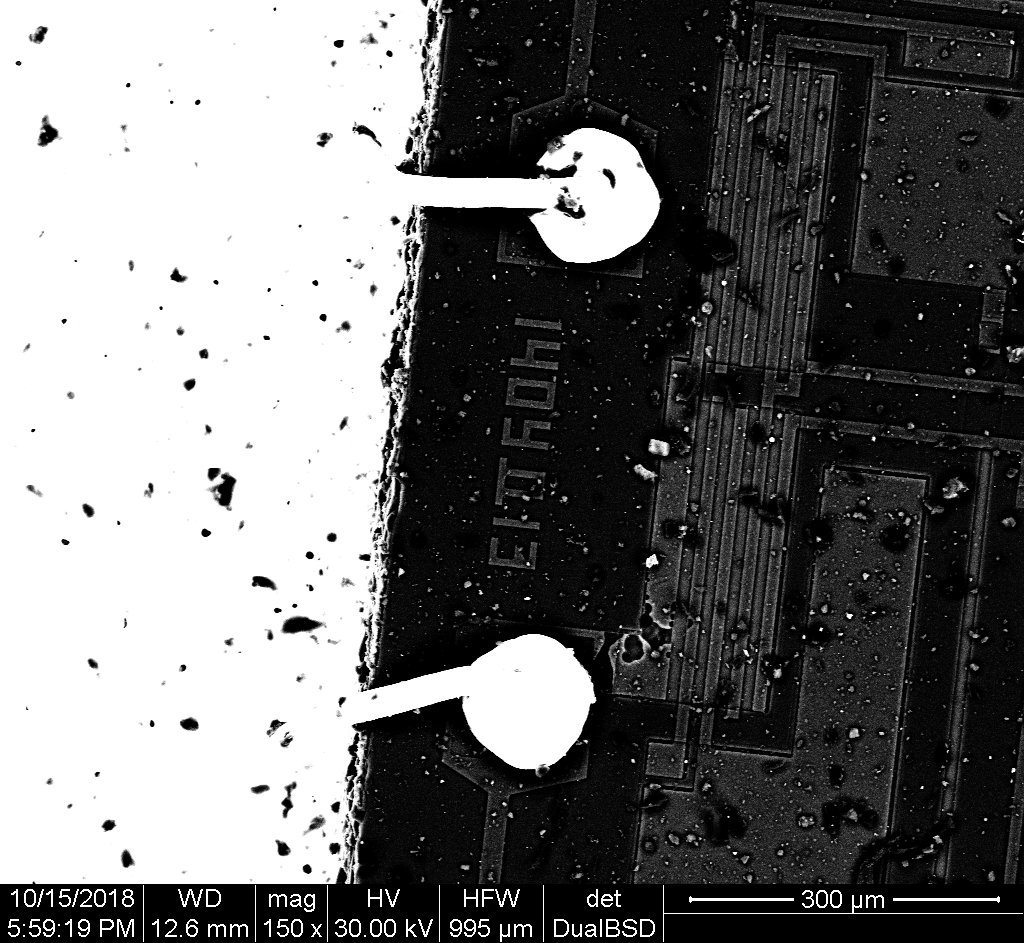
\includegraphics[width=1\linewidth]{z1mikoch_007.jpg}
\caption{Изображение микросхемы (элементный анализ, режим BSE, увеличение 150х)}
\label{ris:experimcoded}
\end{minipage}
\end{center}
\end{figure}

На этих изображениях также видны особенности различных режимов сканирования: более объёмное изображение в режиме SE, более контрастное (без полутонов) - в режиме BSE. Различие изображений, полученных в одном и том же режиме, связано с различным временем выдержки (время сбора электронов детектором при снятии сигнала с одного растра). На изображениях элементного анализа можно увидеть вкрапления другого вещества - лужёные провода, капли припоя (для припоя используются тяжелые металлы, такие как олово, свинец, кадмий - благодаря большому заряду атома на изображении они выглядят светлее.)

\item Создадим в системе низкий вакуум. Получим изображение крыла бабочки в режиме сбора истинно вторичных электронов (рис. 12, 13)

    \begin{figure}[h]
\begin{center}
\begin{minipage}[h]{0.45\linewidth}
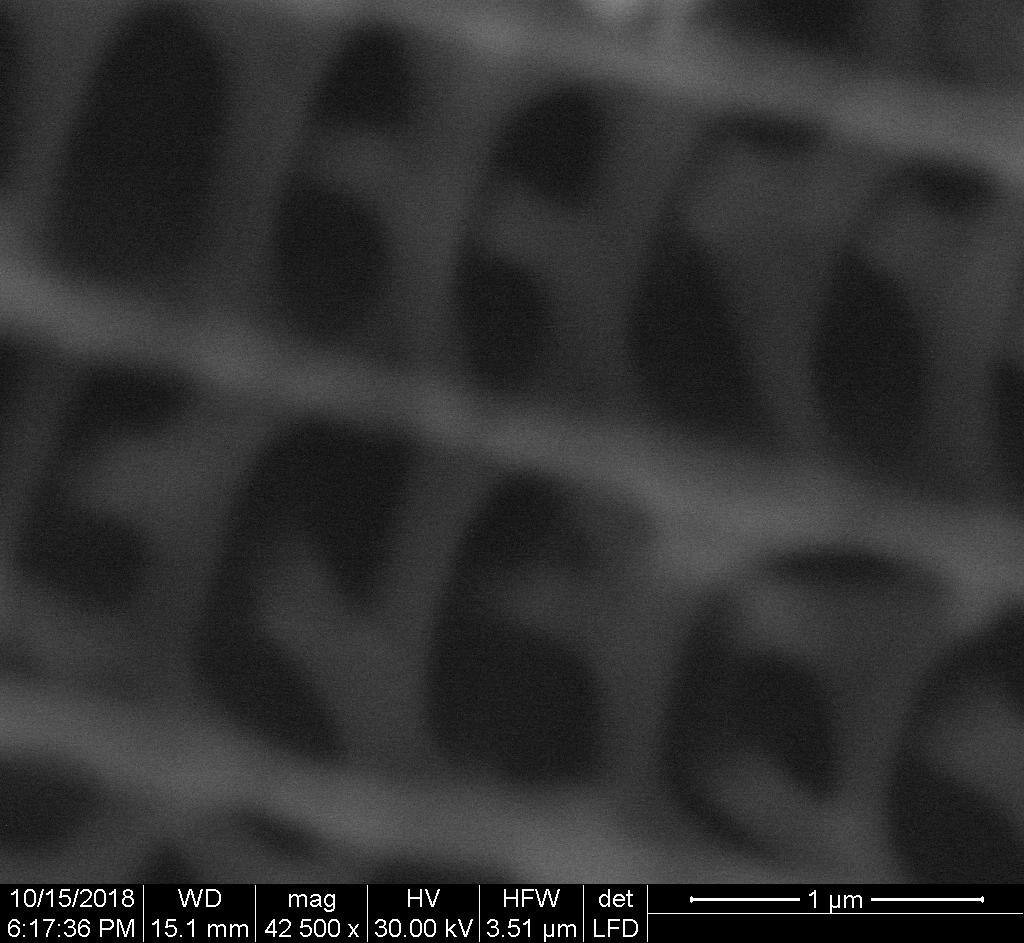
\includegraphics[width=1\linewidth]{iv1bab_006.jpg}
\caption{Изображение крыла бабочки, режим SE, увеличение 42500} %% подпись к рисунку\label{ris:experimoriginal} %% метка рисунка для ссылки на него
\end{minipage}
\hfill 
\begin{minipage}[h]{0.45\linewidth}
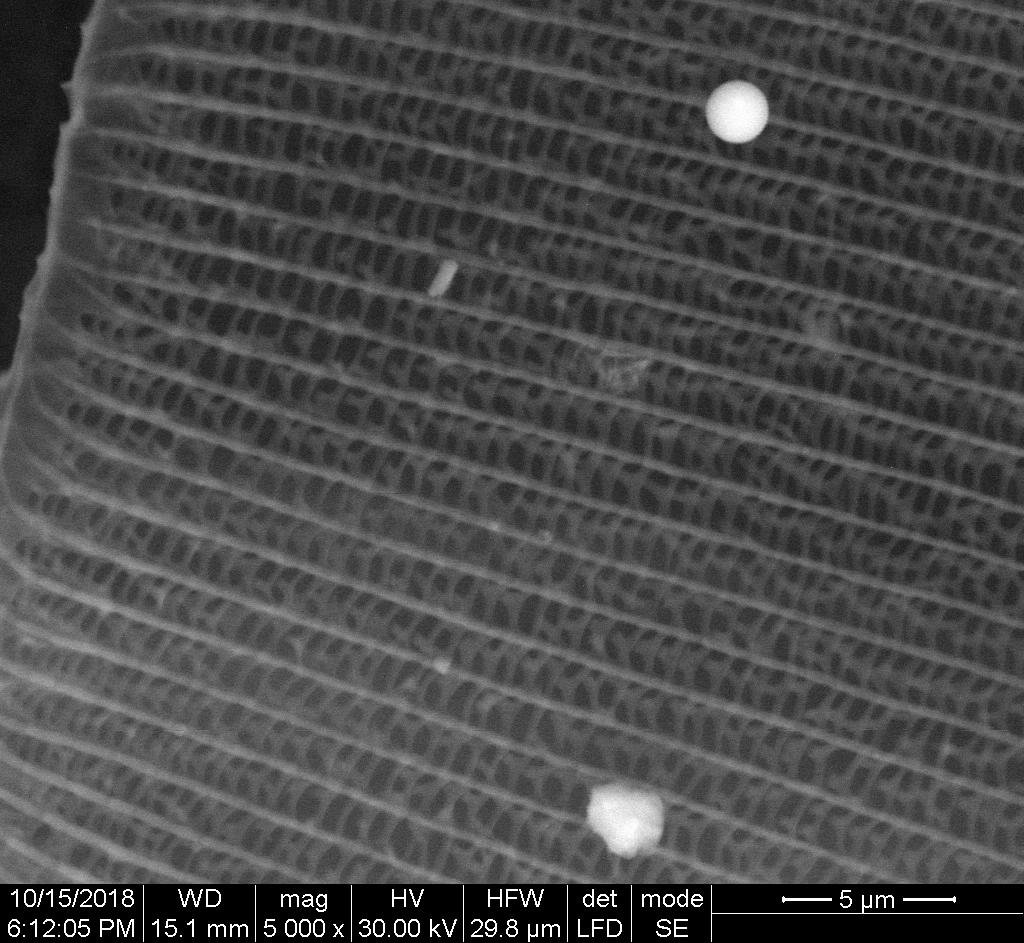
\includegraphics[width=1\linewidth]{iv1bab_005.jpg}
\caption{Изображение крыла бабочки, режим SE, увеличение 5000}
\label{ris:experimcoded}
\end{minipage}
\end{center}
\end{figure}

В режиме сбора истинно вторичных электронов видим объёмное изображение с полутонами.

\clearpage

\item Получим изображение внутренней камеры микроскопа в режимах SE и BSE (рис. 14 - 16)

    \begin{figure}[h]
\begin{center}
\begin{minipage}[h]{0.45\linewidth}
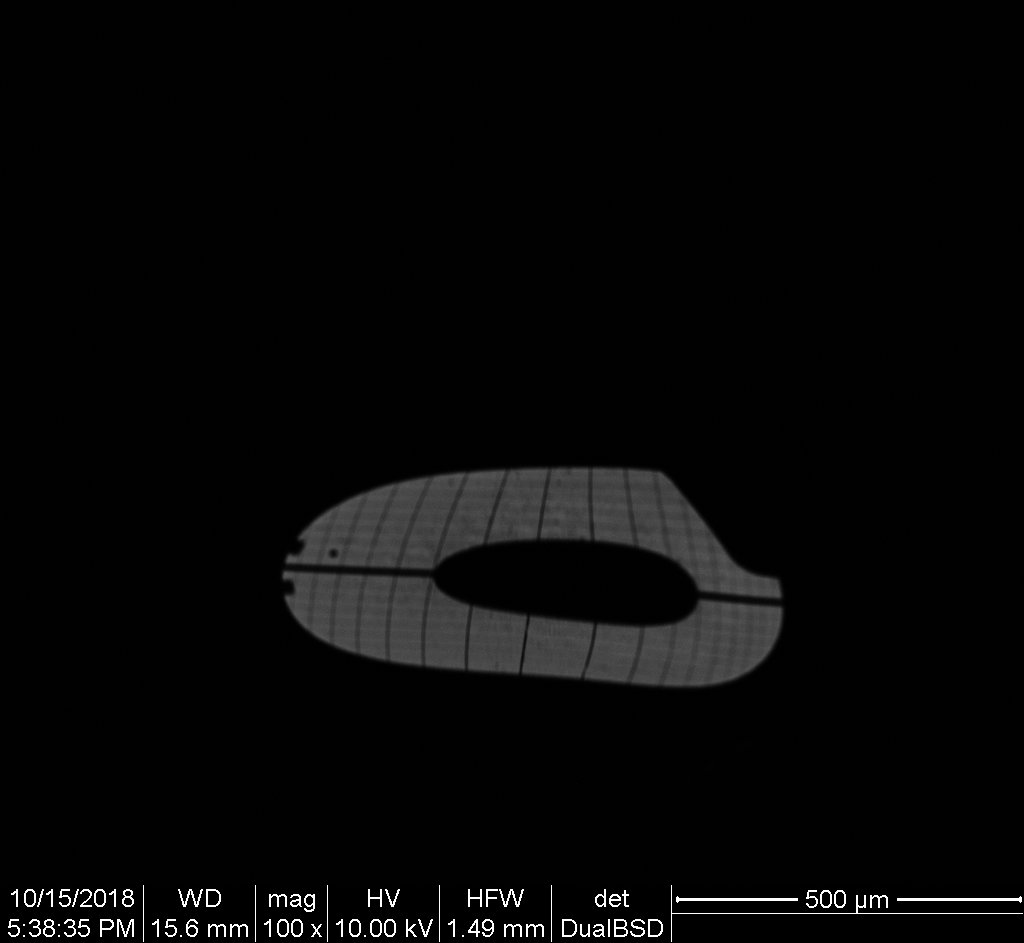
\includegraphics[width=1\linewidth]{z1_002.jpg}
\caption{Изображение внутренней камеры, режим BSE} %% подпись к рисунку\label{ris:experimoriginal} %% метка рисунка для ссылки на него
\end{minipage}
\hfill 
\begin{minipage}[h]{0.45\linewidth}
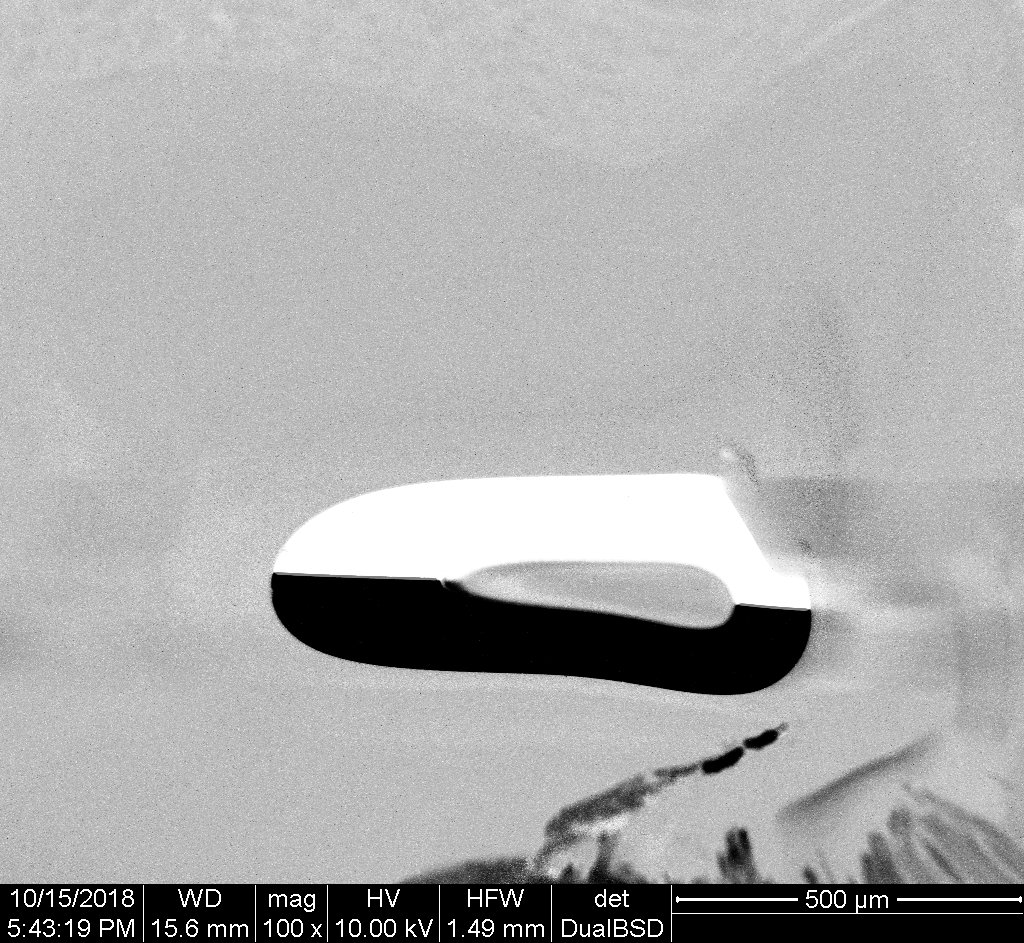
\includegraphics[width=1\linewidth]{z1_003.jpg}
\caption{Изображение внутренней камеры, режим BSE}
\label{ris:experimcoded}
\end{minipage}
\end{center}
\end{figure}

\begin{figure}[h]
\begin{center}
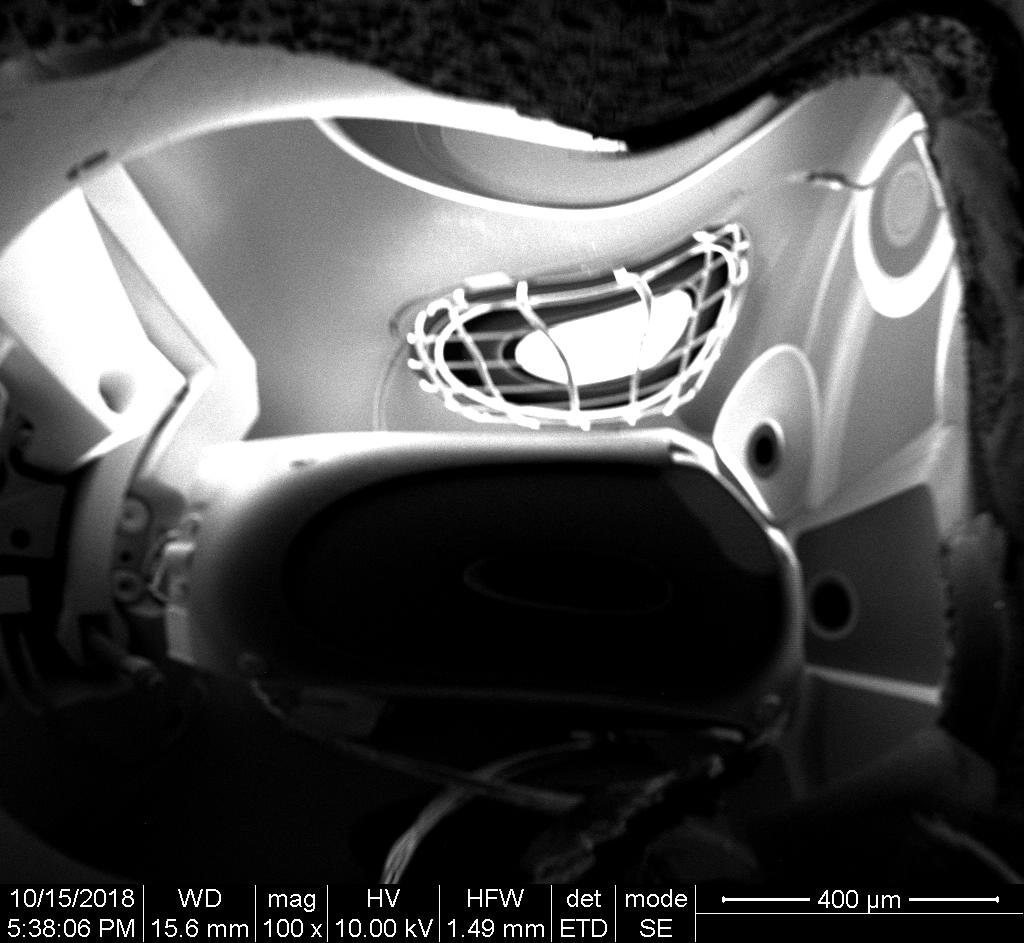
\includegraphics[width=7cm]{iv1_001.jpg}
\caption{Изображение внутренней камеры, режим SE}
\label{ris:experimoriginal} %% метка рисунка для ссылки на него
\end{center}
\end{figure}

Получение изображения внутренней камеры микроскопа возможно благодаря тому, что образец из полистирола при бомбардировке электронами накапливает большой заряд и превращается в электронное
зеркало: электроны после отражения от образца и дальнейшего переотражения от стенок камеры попадают в детектор и образуют изображение камеры микроскопа. На рисунке 12 чётко прослеживается форма детектора отражённых электронов - кольцо, разделённое на две половины, каждая из которых функционирует как отдельный детектор.

\end{enumerate}

\section{Вывод}

В ходе работы были изучены физические принципы работы растрового электронного микроскопа, а также его устройство. Были исследованы образцы сплава медь-хром, микросхемы операционного усилителя, а также крыло бабочки в режиме сбора истинно вторичных электронов, а также в режимах элементного и топографического анализа сбора упругоотражённых электронов.

\end{document}
